% !TEX TS-program = xelatex
% !TEX encoding = UTF-8 Unicode

% Tennessee Technological University
% ENGR1120-021 - GSET - Summer 2021
% Tristan Hill - June 06, 2021
% Module 3 - Operators and Expressions
% Lecture 3 


\documentclass[fleqn]{beamer} % for presentation (has nav buttons at bottom)

%\usepackage{/home/thill/Documents/lectures/cpp_workshop/modules/cpp_lectures}
\usepackage{/mnt/c/Users/thill/Documents/courses/py_workshop/modules/py_lectures}


\newcommand{\MNUM}{3\hspace{2mm}} % Module number
\newcommand{\TNUM}{---\hspace{2mm}} % Topic number - single topic for now
\newcommand{\moduletitle}{Operators and Expressions} % Titles and Stuff
%\newcommand{\topictitle}{---} 

\newcommand{\sectiontitleI}{Operators in Python} % More Titles and Stuff
\newcommand{\sectiontitleII}{Arithmetic Operators}
\newcommand{\sectiontitleIII}{Operator Precedence}
\newcommand{\sectiontitleIV}{What is an Expression?}
\newcommand{\sectiontitleV}{Tutorial 2 - Quadratic Equation - Solution}

\newcommand{\btVFill}{\vskip0pt plus 1filll}

\setbeamercolor{title in head/foot}{fg=TTUgold} % this needs work...

\title{GSET - Intro to Programming with Python}
\author{Tristan Hill\vspc \hspc Tennessee Technological University \hspc}
\date{Summer 2023}

\begin{document}

\lstset{language=MATLAB,basicstyle=\ttfamily\small,showstringspaces=false}

\frame{\titlepage \center\begin{framed}\Large \textbf{Module \MNUM - \moduletitle}\end{framed} \vspace{5mm}}


% Section 0 - Outline
\frame{
	
	\large \textbf{Module \MNUM - \moduletitle} \vspace{3mm}\\
	
	\begin{itemize}
	
		\item \hyperlink{sectionI}{\sectiontitleI} \vspc % Section I
		\item \hyperlink{sectionII}{\sectiontitleII} \vspc % Section II
		\item \hyperlink{sectionIII}{\sectiontitleIII} \vspc %Section III
		\item \hyperlink{sectionIV}{\sectiontitleIV} \vspc %Section IV	
		\item \hyperlink{sectionV}{\sectiontitleV} \vspc %Section V
	
	\end{itemize}

}


% Section I
\section{\sectiontitleI}

	% Section I - Frame I
	\begin{frame}[label=sectionI] \small
		\frametitle{\sectiontitleI}
		
		There are {\it many different} {\BL operators} used in computer programming.  \vspace{5mm}\\
		
		Python Operations, Operators, and Operator Functions  

	    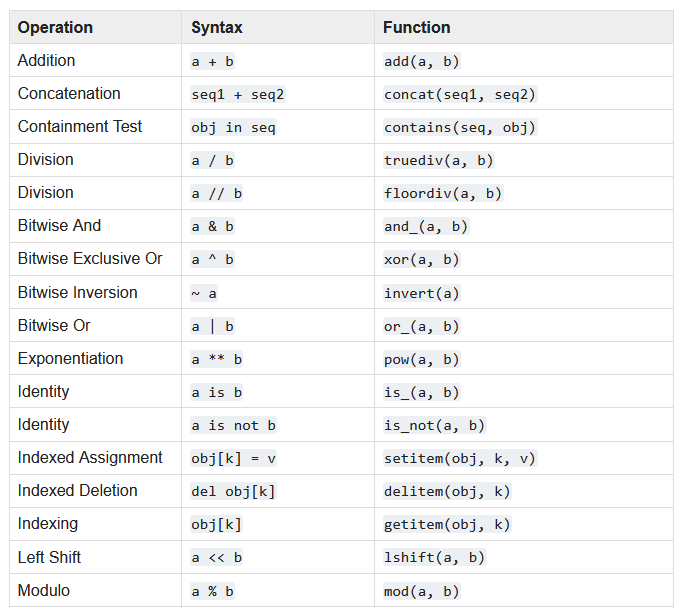
\includegraphics[scale=.375]{operator_list_part1.png}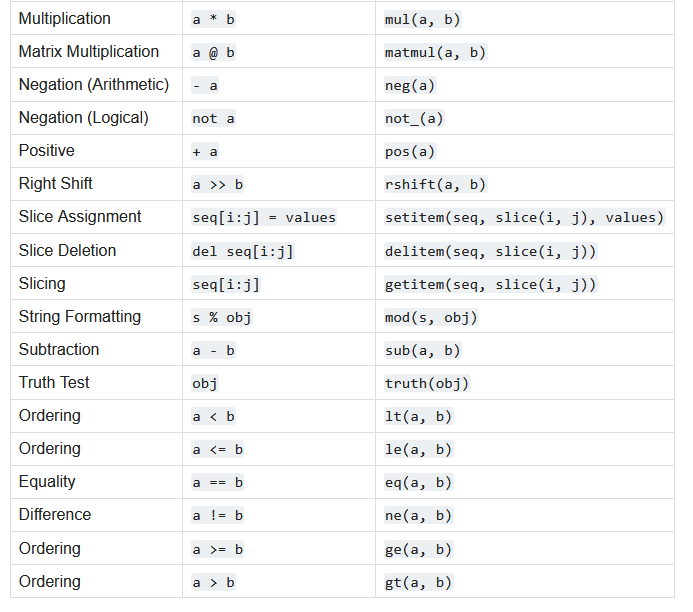
\includegraphics[scale=.375]{operator_list_part2.png}
	
		%\vspace*{10mm}{\tiny See the link below for a complete list of C++ operators.}
		
		\btVFill
		
		\tiny{reference: \href{https://docs.python.org/3/library/operator.html}{docs.python.org} } 	
			
	\end{frame}

	% Section I - Frame II
	\begin{frame} \small
		\frametitle{\sectiontitleI}

			Commonly used operators \vspace{3mm}\\

				\renewcommand*{\arraystretch}{1.5}
		\begin{tabular}{c|c|c} 
			Category&Operators&Example\\ \hline
			Assignment&$=$& \\ \hline
			Arithmetic&$+ \hspc - \hspc * \hspc / \hspc \% \hspcc **$& \\ \hline
			Relational&$== \hspc !\hspace{-1mm}= \hspc > \hspc < \hspc >= \hspc <= $& \\ \hline
			Logical&$! \hspc \&\& \hspc || $& \\ \hline
			Bitwise&$\& \hspc | \hspc \hat{} \hspc \sim \hspc << \hspc >>$ & \\ \hline
		\end{tabular}
		\vspace*{3mm}

        {\it The functions fall into categories that perform object comparisons, logical operations, mathematical operations and sequence operations -python.org}.

		\btVFill
		\tiny{\href{https://docs.python.org/3/library/operator.html}{python.org}}	
	\end{frame}


% Section II
\section{\sectiontitleII}

	% Section II - Frame I
	\begin{frame}[label=sectionII] \small
		\frametitle{\sectiontitleII}
			
		\textbf{Mathematical Operations in Python} \vspace{5mm} \\

		\renewcommand*{\arraystretch}{1.5}
		\begin{tabular}{|c|c|c|} \hline
			\textbf{Operator}& \textbf{Name}& \textbf{Example} \\ \hline
			+ & Addition& x+y \\ \hline
	        - & Subtraction& x-y \\ \hline
	        * & Multiplication& x*y \\ \hline
	        / & Division& x/y \\ \hline
	        \% & Modulus & x\%y \\ \hline
	        ** & Exponentiation & x**y \\ \hline
	        // & Floor Division& x//y \\ \hline 
		\end{tabular} 
	
		\end{frame}

	% Section II - Frame II
	\begin{frame} \small
		\frametitle{\sectiontitleII}
		
		\vspace{5MM}
		
		Which one of these is not like the other?
		
		\vspace{10mm}
		
		{\Large 	$= \hspace{12mm} + \hspace{12mm} - \hspace{12mm} * \hspace{12mm} / \hspace{12mm} \% \hspace{12mm} **$ }
		
		\vspace{10mm}
		
		Why?
		
		\btVFill
		\tiny{ref: \href{some link}{some text}}
	\end{frame}	


% Section III
\section{\sectiontitleIII}

	% Section III - Frame I
	\begin{frame}[label=sectionIII] \small
		\frametitle{\sectiontitleIII}
		
		\begin{multicols}{2}
		The intepretter must assume an order to perform operations. The {\it operator precedence} for python is shown in the table. The top of the table has highest precedence.

		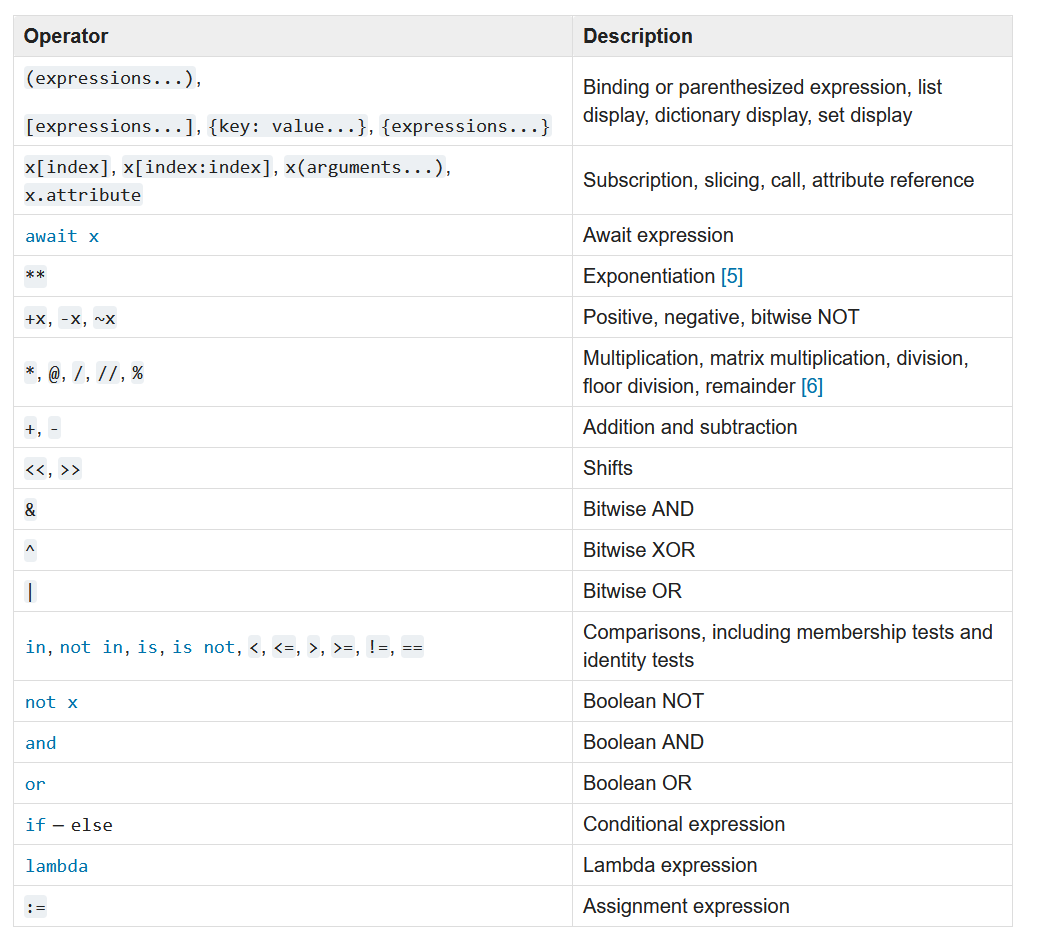
\includegraphics[scale=.275]{operator_precedence_python.png}
		
		\end{multicols}
		\btVFill
		\tiny{reference: \href{https://docs.python.org/3/reference/expressions.html\#expression-lists}{python.org} }

	\end{frame}

	% Section III - Frame II
	\begin{frame} \small
		\frametitle{\sectiontitleIII}
		
		\underline{Question:} What was the concept of operator precedence called in mathematics class? \vspace{15mm}
		
		\underline{Answer:}
		
	\end{frame}


% Section IV
\section{\sectiontitleIV}	
	% Section IV - Frame I
	\begin{frame}[label=sectionIV] \small
		\frametitle{\sectiontitleIV}    
	
		\vspace{15mm}
	
		{\it An expression is a sequence of operators and their operands, that specifies a computation.}

		\btVFill
		\tiny{reference: \href{https://www.cplusplus.com/doc/tutorial/operators/}{cplusplus.com} } 
	\end{frame}

% Section V
\section{\sectiontitleV}	
	% Section V - Frame I
	\begin{frame}[label=sectionV,containsverbatim] \small
	\frametitle{\sectiontitleV}    
	

	\end{frame}


\end{document}

